\documentclass[red]{beamer}
\usepackage{beamerthemelined} 
\usepackage{amsmath}
\usepackage[utf8x]{inputenc}
\usepackage{tikz}
\usepackage{graphicx}
\usepackage{epsfig}
\usepackage{color}
\usepackage{tikz}
\usepackage{hyperref}
\usepackage{amsthm}

\newcommand*\arc{{\fontfamily{pbk}\fontseries{db}\selectfont+}}

\usetheme{Warsaw}
\usecolortheme{crane}
\usepackage{pgf}  

\title{Problém šachového ťahu a derivácie polynómu}
\author{Adam Krupička, Matej Troják}                 
\institute{FI MUNI}      
\date{17th December 2015}            

\begin{document}
\begin{frame}
  \titlepage
\end{frame}

\section{Problém šachového ťahu}

\begin{frame}
\frametitle{Zdroj dát} 
\begin{center}
\begin{minipage}{0.4\textwidth}
\begin{center}
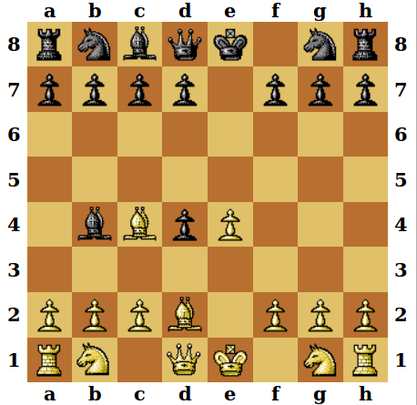
\includegraphics[scale=0.25]{from}
\end{center}
\end{minipage}%
\begin{minipage}{0.1\textwidth}
\begin{center}
$\longrightarrow$
\end{center}
\end{minipage}
\begin{minipage}{0.4\textwidth}
\begin{center}
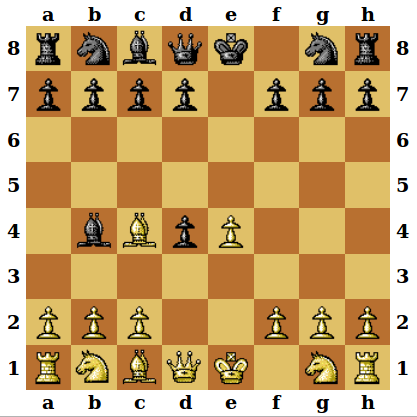
\includegraphics[scale=0.25]{to}
\end{center}
\end{minipage}
\begin{itemize}
\item sme záznamy šachových partií z Games of World Champions
\item prevedené do formátu FEN (Forsyth–Edwards Notation)
\item cca. 2 milióny ťahov 
\end{itemize}
\end{center}
\end{frame}

\begin{frame}
\frametitle{Prístupy} 
\begin{center}
\begin{itemize}
\item vstupná šachovnica $\rightarrow$ vystupná šachovnica

\vspace*{0.2cm}
\begin{minipage}{.5\textwidth}
\begin{center}
{\small
\begin{tabular}{| l l | l l |}
\hline
 pešiak & 1 & strelec & 4 \\
 veža & 2 & kráľ & 5 \\
 kôň & 3 & kráľovná & 6\\
\hline
\end{tabular}
}
\end{center} 
\end{minipage}%
\begin{minipage}{.5\textwidth}
$F_a(x)=12 \times tanh(\frac{x}{12})$
\end{minipage}%
\begin{itemize}
\item sekvencia 64 číslic v rozsahu [-6, 6]
\end{itemize}

\item pozície jednotlivých figúrok $ \rightarrow $ zmenené pozície

\begin{minipage}{.5\textwidth}
\begin{itemize}
\item sekvencia 64 číslic v rozsahu [0,~8] -- pozície fixne daného poradia figúrok
\end{itemize}
\end{minipage}%
\begin{minipage}{.5\textwidth}
\[ F_a(x) =
  \begin{cases}
    \quad 0  & \quad x \leq 0 \\
    \quad x  & \quad x > 0\\
  \end{cases}
\]
\end{minipage}%

\item pozície jednotlivých figúrok $ \rightarrow $ zmena na šachovnici

\begin{itemize}
\item dve dvojice (from$_x$, from$_y$), (to$_x$, to$_y$)
\end{itemize}

\end{itemize}
\end{center}
\end{frame}

\section{Problém derivácie polynómu}

\begin{frame}
\begin{center}
\hspace*{0.5cm}\begin{minipage}{\textwidth}
\textbf{Zdroj dát}
\begin{itemize}
\item funkcia generujúca náhodné polynómy
\end{itemize}
\textbf{Maximálny stupeň polynómu}
\begin{itemize}
\item vstupný ponynóm obmedzený
\item závislosť počtu vstupných neurónov na dĺžke polynómu
\end{itemize}
\end{minipage}
\end{center} 
\end{frame}

\begin{frame}
\begin{center}
\frametitle{Reprezentácia}
\begin{itemize}
\item vstup: sekvencia čísel `8 2 0 5 0 0'
\begin{itemize}
\item t.j. polynóm $f(x)=5x^3 + 2x + 8$
\item chápaný ako $f(x)= {\color{red} 8} x^0 + {\color{red} 2}x^1 + 0x^2 + {\color{red} 5}x^3 + 0x^4 + 0x^5$
\end{itemize}

\vspace*{1cm}

\item výstup: sekvencia čísel `2 0 15 0 0'
\begin{itemize}
\item t.j. polynóm $f'(x)=2 + 15x^2$
\item chápaný ako $f'(x)={\color{red} 2}x^0 + 0x^1 + {\color{red} 15}x^2 + 0x^3 + 0x^4$
\end{itemize}
\end{itemize}
\end{center} 
\end{frame}

\begin{frame}
\frametitle{Parametre siete}
\begin{center}
\begin{itemize}
\item lineárna aktivačná funckcia: $F_a(x)=x$
\item topológia minimálna (pre 5 vstupov):
\end{itemize}

\vspace*{0.5cm}
\includegraphics[scale=0.3]{net}

\begin{itemize}
\item rýchlosť učenia -- 0.0001
\item učenie \textit{po stĺpcoch} 100 tisíc polynómoch
\end{itemize}
\end{center} 
\end{frame}

\begin{frame}
\frametitle{Výsledky}

\vspace*{0.5cm}

\begin{tabular}{ l l }
		vstup: & $20.5x^1$~\arc~$11.3x^2$~\arc~$2.5x^3$~\arc~$-0.5x^4$\\
		výstup: & $20.48$~\arc~$22.5747x^1$~\arc~$7.46458x^2$~\arc~$-2.04699x^3$
\end{tabular}

\vspace*{1cm}

\begin{tabular}{ l l }
		vstup: & $20.5x^1$~\arc~$11.3x^2$~\arc~$20x^3$~\arc~$-500x^4$\\
		výstup: & $20.7582$~\arc~$23.0364x^1$~\arc~$60.6112x^2$~\arc~$-1999.19x^3$
\end{tabular}

\end{frame}

\end{document}